\section{17 靶点的探索性支持结果}

\subsection{天然复合物集合不能评价甲基阳性召回}

17 个天然复合物共包含251个选中短肽位点；天然结构的序列评价保留预先选定的全部短肽链，部分靶点因此贡献多条等价肽链，而生成结构评价只使用单条预测末链。天然化基础序列恢复为 53/251（21.12\%）。这251个真值位点全部是未甲基化阴性，因此 ROC-AUC、Precision、Recall 和 F1 都没有阳性类别可供计算；若给出这些数字，数学上没有意义。阈值严格 $p>0.6$ 时，已知天然序列条件产生 19 个假阳性（19/251，7.57\%），端到端条件产生 9 个预测甲基位点（9/251，3.59\%）。后一个比例同时受基础氨基酸预测错误影响，不能解释为甲基化头单独的假阳性率。

\begin{table}[H]
\centering
\caption{17 个天然复合物上的可报告序列指标。所有甲基化真值均为阴性。}
\label{tab:native17}
\begin{tabular}{L{47mm}C{29mm}C{29mm}L{44mm}}
\toprule
指标 & 计数 & 比例 & 解释 \\
\midrule
天然化 RAA & 53/251 & 21.12\% & 基础氨基酸恢复 \\
已知序列甲基假阳性 & 19/251 & 7.57\% & 真阴性集合上的 FPR \\
端到端预测甲基位点 & 9/251 & 3.59\% & 含基础类别级联误差 \\
AUC/Precision/Recall/F1 & \NA & 不可定义 & 没有甲基阳性真值 \\
\bottomrule
\end{tabular}
\end{table}

\subsection{五个温度的生成覆盖与重复率}

原始全温度文件共有 4015 条记录；分别在每个温度内去重后合计 3443 条。比较两个端点，温度内唯一率在 $T=0.01$ 与0.5时分别为78.05\%和94.88\%，平均天然序列恢复分别为1.49\%和4.42\%，平均甲基标记率分别为27.69\%和9.67\%（\cref{tab:alltemp}）。其中唯一率在 $T=0.1$ 降至74.37\%，所以这些变化并非全程单调。它们是生成池的描述统计，不是独立同分布实验重复，也不能把不同温度的样本量差异解释为温度效应的因果证据。

\begin{table}[H]
\centering
\caption{17 靶点原始生成池的温度分层统计。唯一数是在各温度内去重；甲基标记率为序列内小写甲基 token 比例的均值。}
\label{tab:alltemp}
\begin{tabular}{C{15mm}rrrrrr}
\toprule
$T$ & 原始数 & 唯一数 & 重复数 & 唯一率 & 平均 RAA & 平均甲基率 \\
\midrule
0.01 & 82   & 64   & 18  & 78.05\% & 1.49\% & 27.69\% \\
0.10 & 394  & 293  & 101 & 74.37\% & 2.46\% & 23.24\% \\
0.20 & 776  & 597  & 179 & 76.93\% & 3.52\% & 19.87\% \\
0.30 & 1181 & 988  & 193 & 83.66\% & 3.90\% & 15.54\% \\
0.50 & 1582 & 1501 & 81 & 94.88\% & 4.42\% & 9.67\% \\
\midrule
合计 & 4015 & 3443 & 572 & 85.75\% & \NA & \NA \\
\bottomrule
\end{tabular}
\end{table}

\subsection{best85：肽内部形状尚可，但结合姿态普遍偏离}

旧 best85 队列覆盖 $17\times5=85$ 个靶点--温度组合，结构文件和链映射均为 85/85。由于每个组合的代表是按真实天然序列恢复率从多个候选中选出，这一队列是选择条件化的 oracle 集合；它回答“知道天然答案后所挑代表的表现”，不回答一次盲生成的期望表现。

在受体框架对齐后，肽 CA RMSD 的均值/中位数为 29.93/40.06~\AA，肽 backbone RMSD 为 29.83/39.96~\AA；CA RMSD $<2$~\AA 为 0/85，$<5$~\AA 为 3/85（3.53\%）。相反，单独对肽自身拟合后，CA 与 backbone RMSD 的均值/中位数分别为 2.65/2.53~\AA 和 2.34/2.11~\AA（\cref{tab:best85-rmsd}）。这组巨大差异说明，部分序列可形成与天然肽相似的内部形状，但没有位于正确的受体结合位置；因此不能用肽自对齐 RMSD 宣称设计成功。

\begin{table}[H]
\centering
\caption{best85 的旧结构评价。受体框架对齐反映结合姿态；肽自对齐仅反映内部形状。}
\label{tab:best85-rmsd}
\begin{tabular}{L{58mm}C{20mm}C{23mm}C{29mm}}
\toprule
指标 & $n$ & 均值（\AA） & 中位数（\AA） \\
\midrule
受体拟合后肽 CA RMSD & 85 & 29.930 & 40.064 \\
受体拟合后肽 backbone RMSD & 85 & 29.835 & 39.960 \\
肽自拟合 CA RMSD & 85 & 2.647 & 2.530 \\
肽自拟合 backbone RMSD & 85 & 2.342 & 2.105 \\
\bottomrule
\end{tabular}
\end{table}

best85 共含 159 个模型标记的甲基位点和 626 个非甲基位点。按两组坐标平方和合并后开方得到的 pooled CA RMSD，在受体拟合后分别为20.43与34.18~\AA，在肽自拟合后分别为3.28与2.93~\AA；这些数值不是逐设计或逐位点 RMSD 的算术均值。由于位点是否甲基化本身由模型选择，并同时关联残基类别、靶点、温度和结构可解析性，这只是选择后的描述，不能推出“甲基化导致更好结合姿态”或其他因果关系。

\subsection{多样性、置信度、通透性和 fixed-pose 分数}

同一靶点的五个温度代表进行两两比较，共得到170对。对称 TM-score 的均值与中位数分别为0.340和0.309；对应多样性 $1-\mathrm{TM}$ 分别为0.660和0.691，提示代表结构之间存在较大内部形状差异。但它既受温度影响，也受 oracle 挑选影响，不等价于完整生成分布的多样性。

结构 PDB 的 CA B-factor 代理在 85/85 条中可用，均值为 87.55。HighFold COMMENT 的 global pLDDT、肽链 pLDDT、pTM 和受体--肽 ipTM/PAE 字段仅在 37/85 条中存在；在这些可用条目中，global pLDDT、肽链 pLDDT、pTM 与受体--肽 ipTM 的均值分别为 71.07、46.53、0.146 和 0.461，肽链内 PAE、链间 PAE 与界面 PAE 的均值分别为 3.64、18.05 和 12.14。缺失的 48 条不能填零，PDB B-factor 代理也不能替代 COMMENT 字段。

预测通透性在85/85条中有数值：82条由靶点、序列和温度严格匹配，3条（3WNE 的 $T=0.01/0.1$ 与3ZGC的 $T=0.1$）因同一序列跨温度重复而回填，故温度分层图包含这项来源限制。总体中位数为 $1.84\times10^{-8}$（模型单位）；两个端点 $T=0.01$ 与0.5的中位数分别为 $3.17\times10^{-9}$ 与 $5.16\times10^{-6}$，但 $T=0.1$ 为 $2.43\times10^{-9}$，并非全程单调。由于没有实验通透性标签，这只能视为模型预测分布，不能报告准确率或外部验证结论。

自然化 fixed-pose PyRosetta 评分覆盖 85/85 条。复合物每残基分数的中位数为 1.799~REU，cross-interface 分数的均值/中位数为 259.97/110.07~REU，只有 6/85 为负。该流程没有在同一参数化、同一优化协议下计算天然参考，也没有显式 N-甲基残基参数；因此无法计算“低于天然能量”的 success 或 stability，更不能把这些数值称为结合自由能。

\begin{figure}[H]
  \centering
  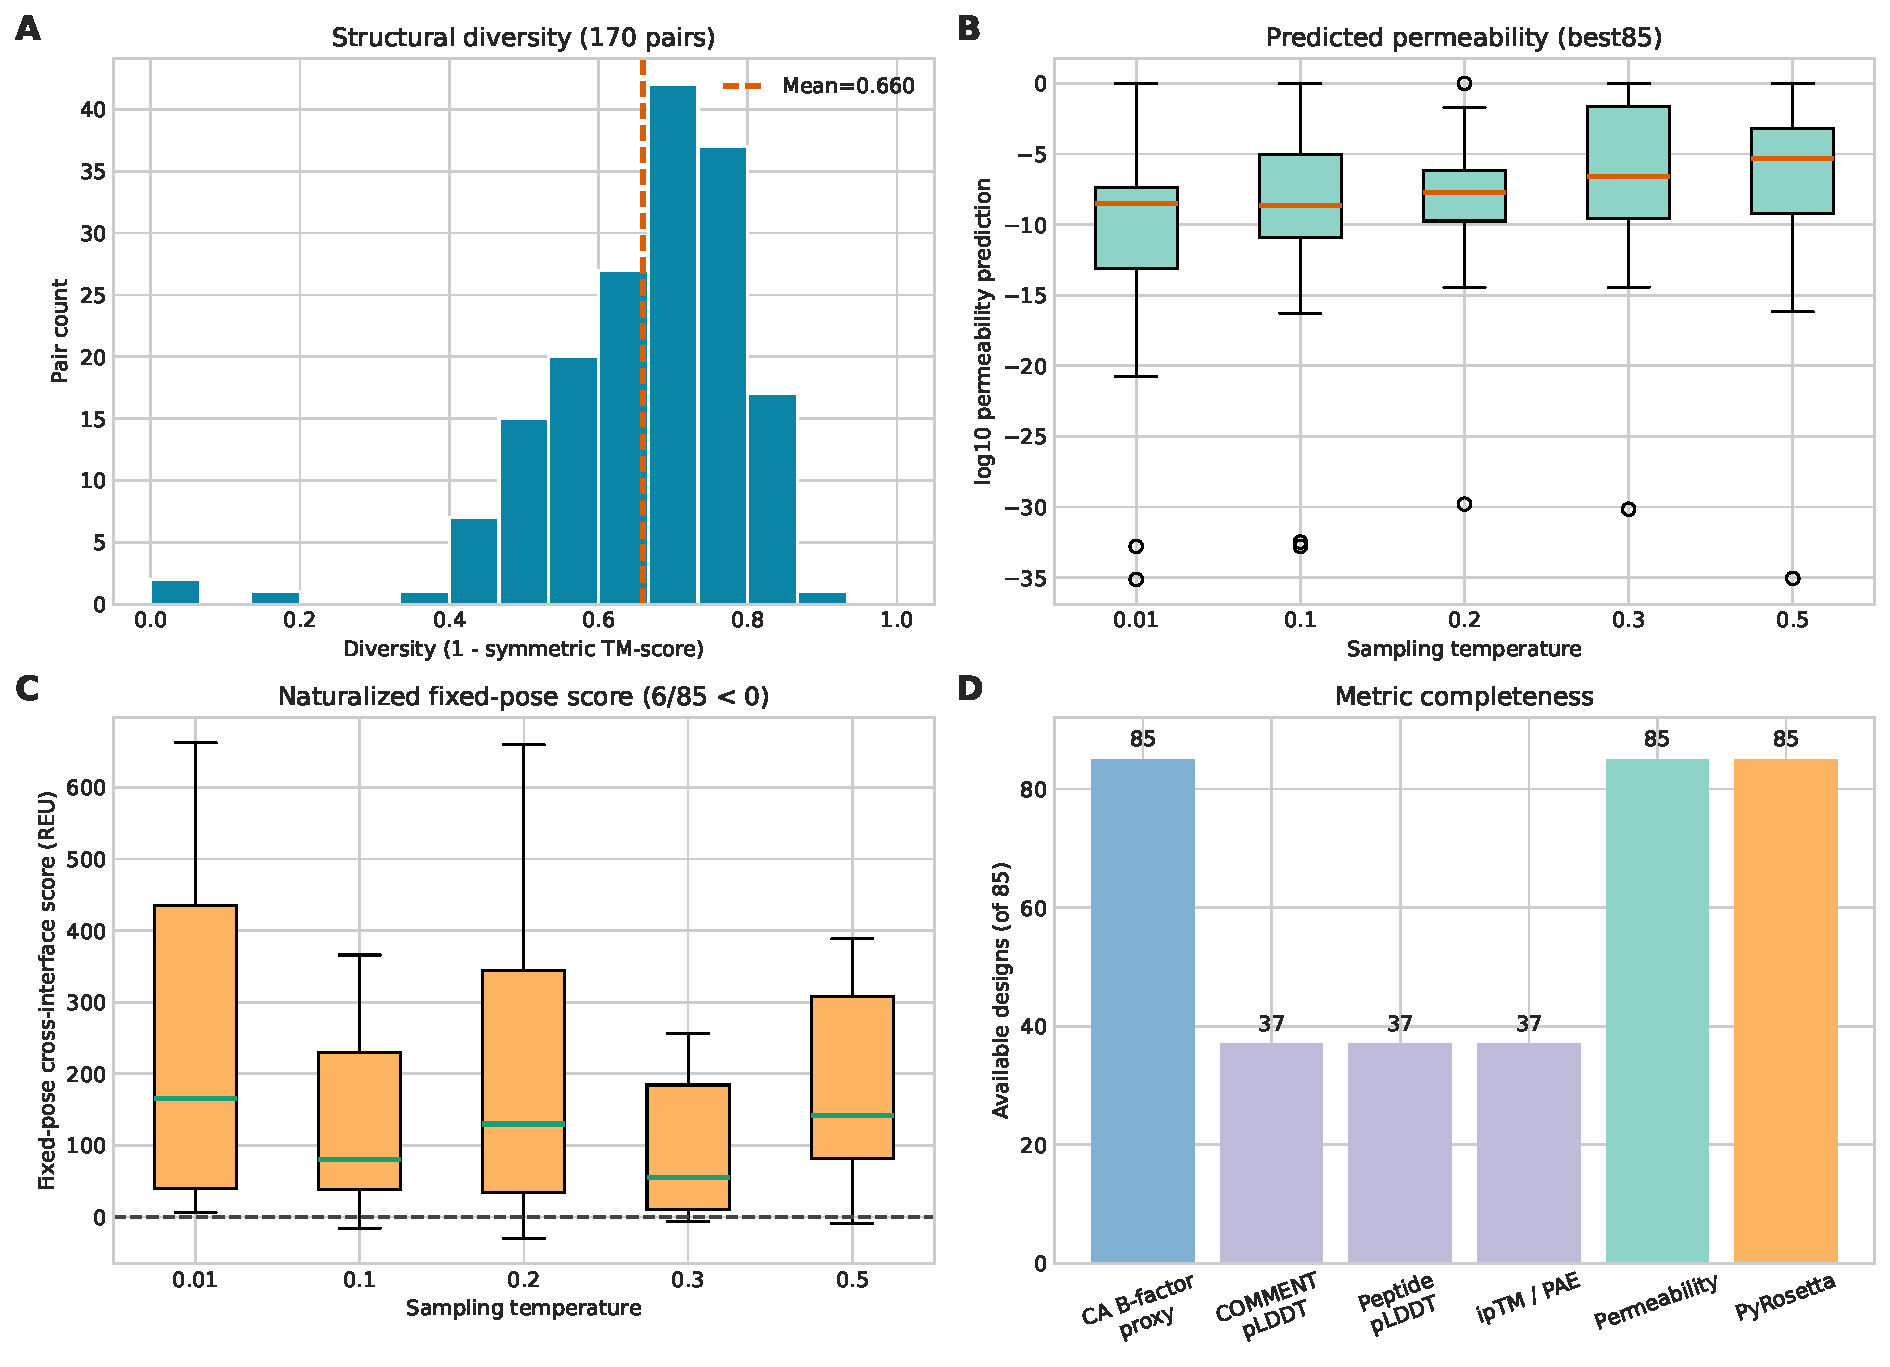
\includegraphics[width=0.98\textwidth]{figures/Fig6_best85_exploratory_support.pdf}
  \caption{17 靶点 best85 的探索性支持结果。A，靶点内五温度代表的 $1-\mathrm{TM}$ 分布；B，按温度分层的通透性预测，其中3条为相同序列的跨温度回填；C，自然化 fixed-pose cross-interface Rosetta 分数；D，各指标的文件可用数。所有面板均受 oracle 选择影响，不能替代六复合物的预设主分析。}
  \label{fig:best85}
\end{figure}
